\documentclass[10pt]{article}
\usepackage{kotex}
\usepackage[margin=0.6in]{geometry} % set the margins to 1in on all sides
\usepackage{graphicx} % to include figures
\usepackage{amsmath} % great math stuff
\usepackage{amsfonts} % for blackboard bold, etc
\usepackage{amsthm} % better theorem environments
\usepackage{amssymb}
\usepackage[utf8]{inputenc}
\usepackage{booktabs}
\usepackage{array}
\usepackage{courier}
\usepackage[usenames, dvipsnames]{color}
\usepackage{titlesec}
\usepackage{empheq}
\usepackage{tikz}
\usepackage{wrapfig}
\usepackage{float}
\usepackage{algorithm}
\usepackage{algpseudocode}
\usepackage{tikz}

\linespread{1.5}

\newcommand\tikzmark[1]{%
  \tikz[remember picture,overlay]\node[inner sep=2pt] (#1) {};}
\newcommand\DrawBox[3][]{%
  \tikz[remember picture,overlay]\draw[#1] ([xshift=-3.5em,yshift=7pt]#2.north west) rectangle (#3.south east);}

\algnewcommand\algorithmicinput{\textbf{Input:}}
\algnewcommand\INPUT{\item[\algorithmicinput]}
\newcommand\encircle[1]{%
  \tikz[baseline=(X.base)] 
    \node (X) [draw, shape=circle, inner sep=0] {\strut #1};}
 
% Command "alignedbox{}{}" for a box within an align environment
% Source: http://www.latex-community.org/forum/viewtopic.php?f=46&t=8144
\newlength\dlf  % Define a new measure, dlf
\newcommand\alignedbox[2]{
% Argument #1 = before & if there were no box (lhs)
% Argument #2 = after & if there were no box (rhs)
&  % Alignment sign of the line
{
\settowidth\dlf{$\displaystyle #1$}  
    % The width of \dlf is the width of the lhs, with a displaystyle font
\addtolength\dlf{\fboxsep+\fboxrule}  
    % Add to it the distance to the box, and the width of the line of the box
\hspace{-\dlf}  
    % Move everything dlf units to the left, so that & #1 #2 is aligned under #1 & #2
\boxed{#1 #2}
    % Put a box around lhs and rhs
}
}


\newtheorem{thm}{Theorem}[section]
\newtheorem{lem}[thm]{Lemma}
\newtheorem{prop}[thm]{Proposition}
\newtheorem{cor}[thm]{Corollary}
\newtheorem{conj}[thm]{Conjecture}

\setcounter{secnumdepth}{4}

\titleformat{\paragraph}
{\normalfont\normalsize\bfseries}{\theparagraph}{1em}{}
\titlespacing*{\paragraph}
{0pt}{3.25ex plus 1ex minus .2ex}{1.5ex plus .2ex}

\definecolor{myblue}{RGB}{72, 165, 226}
\definecolor{myorange}{RGB}{222, 141, 8}

\setlength{\heavyrulewidth}{1.5pt}
\setlength{\abovetopsep}{4pt}


\DeclareMathOperator{\id}{id}
\DeclareMathOperator{\argmin}{\arg\!\min}
\DeclareMathOperator{\Tr}{Tr}

\newcommand{\bd}[1]{\mathbf{#1}} % for bolding symbols
\newcommand{\RR}{\mathbb{R}} % for Real numbers
\newcommand{\ZZ}{\mathbb{Z}} % for Integers
\newcommand{\col}[1]{\left[\begin{matrix} #1 \end{matrix} \right]}
\newcommand{\comb}[2]{\binom{#1^2 + #2^2}{#1+#2}}
\newcommand{\bs}{\boldsymbol}
\newcommand{\opn}{\operatorname}
\begin{document}
\nocite{*}

\title{$\pi$의 정확한 의미와 그에 대한 실용적 고찰}
\author{임대영 \\ 고려대학교 통계학과}
\maketitle

\section{$\pi$는 존재하지 않는다}
통계를 조금 공부해보면 다음과 같은 질문이 자주 생기게 된다. `실제로 정규 분포를 따르는 것이 있을까?' 통계 질문방에 가봐도 ``아이비리그에 들어가는 것은 확률과정인가요?'' 혹은 ``학생들의 성적은 정규분포인가요?''와 같은 질문이 수도 없이 많다. 이런 질문이 올라올 때마다 나의 답변은 ``이 세상에 존재하는 그 어떤 것도 확률과정이거나 정규분포를 따르는 것은 없습니다''이다. 수학을 공부하는 사람들이 가장 많이 하는 착각이 바로 이런 것이다. 수학 책에 나오는 모든 것들이 실재할 것이라는 착각. 물론 직관적으로 이해가 잘 되는 것은 있다. 자연수가 대표적이다. 이 때문에 레오폴트 크로네커(Leopold Kronecker)라는 과거 프로이센의 수학자는 다음과 같이 말하기도 했다.
\begin{center}
  ``정수는 신이 만들었지만 나머지는 인간의 창작물이다.'' (God made the integers. All else is the work of man.)
\end{center}
 `수'라는 것은 인간의 위대한 발명품이지만 실제로 존재하지는 않는다. 상당히 철학적이다. 숫자가 존재하지 않는다니! 하지만 잘 생각해보면 숫자라는 건 실재하는 것이 아니라 사람이 쓰기 좋게 만들어놓은 하나의 도구라는 것이 명료해질 것이다. 자꾸 이런 직관에 의존하려고 하다보니 어차피 다 실존하지 않는 창작물인데 유독 `허수'에만 허구라는 꼬리표를 달아놓는다. 하지만 허수를 포함한 복소수도 매우 직관적으로 이해할 수 있는 것들이며 그와 동시에 존재하지 않으면서도 많은 현상과 운동, 법칙을 설명할 수 있는 좋은 도구이다. 이러한 특성은 $\pi$라고 예외일 수 없다. 매우 충격적인 사실은 물리적인 형체를 지니고 있는 이 세상의 그 어떤 원도 원주와 지름의 비율이 정확히 $\pi$가 아니다. 모든 물리적인 측정에는 오차가 따른다. 다시 한 번 강조하지만 정확히 $\pi$의 값을 지니는 것은 없다. 있다고 해도 우리는 무엇이 `정확히' $\pi$의 값을 지니는지 알 턱이 없다. $\pi$는 없다.
\section{$\pi$ 원주율이 아니다}
\begin{wrapfigure}{r}{0.2\textwidth}
  \centering
  
\includegraphics[width = 0.2\textwidth]{exp_mosaic.png}
  \caption{Mosaic image of $\exp\left(ix\right)$}
\end{wrapfigure}\par
$\pi$를 처음 배울 때 그 누구나 다 `원주율'이라고 배웠다. 반은 맞고 반은 틀렸다. 유클리드 기하에서는 원의 곡률이 0이고 원주와 지름의 비율이 $\pi$라는 상수가 된다. 하지만 쌍곡 기하에서는 곡률이 음수가 되며 원이 커지면 커질수록 원주와 지름의 비율은 무한대로 증가한다. 따라서 어떤 상수로 정의될 수 없다. 타원 기하에서도 마찬가지로 곡률이 양수이며 원주와 지름의 비율이 원이 커짐에 따라 감소한다. 여기서도 상수가 아니다. 그러면 $\pi$는 원주율이라고 정의할 때는 유클리드 기하를 전제하고 하는 말일 것이다. 무엇을 정의할 때 전제가 필요한 것과 전제가 필요없는 것이 있다면, 오컴의 법칙(Occam's razor)에 따라 전제가 필요없는 것을 따라야 할 터이다. 그렇다면 이러한 정의는 어떻게 할 수 있을까?\par
오른쪽에 있는 것은 복소지수함수의 모자이크 이미지이다. 패턴이 보이는가? 그렇다면 $\pi$의 흔적을 찾은 것이다. 조금 더 명확하게 보고 싶다면 아래의 그래프를 보자. 

% 한국에서 고등 교육을 받은 사람이라면 $\pi$를 모르는 사람은 없을 것이다. 하지만 매일 $\pi$를 써서 계산을 해 내는 물리학자나 수학자도 $\pi$에 대해 설명하라고 하면 단박에 그 정수를 찔러 설명하지 못할 듯싶다. 그토록 이 숫자에는 아주 중요한 성질이 있고 그것은 한 마디로 표현하기에는 너무 중요하다.\par
% $\pi$는 원주율이다. 분명 이 숫자는 원과 관련이 있다. 그러나 이러한 정의는 `틀렸다'고 할 수 있을 정도로 그 본질을 설명하지 못한다. $\pi$는 원이나 각도 따위를 알지 못한다. 예를 들어, 통계학에서 가장 중요한 정규 분포의 밀도 함수에 등장하는 $1/\sqrt{2\pi}$에서 원의 흔적을 발견할 수 있는가? 원의 성질과 연결시키지 않아도 우리는 충분히 정규 분포의 중요성을 설명할 수 있다. 왜냐하면 $\pi$는 원에서 나온 숫자가 아니기 때문이다. $\pi$는 원과 관련짓지 않고도 그 중요성을 명료하게 설명할 수 있는 숫자이다.\par
\begin{wrapfigure}{l}{0.5\textwidth}
  \centering
  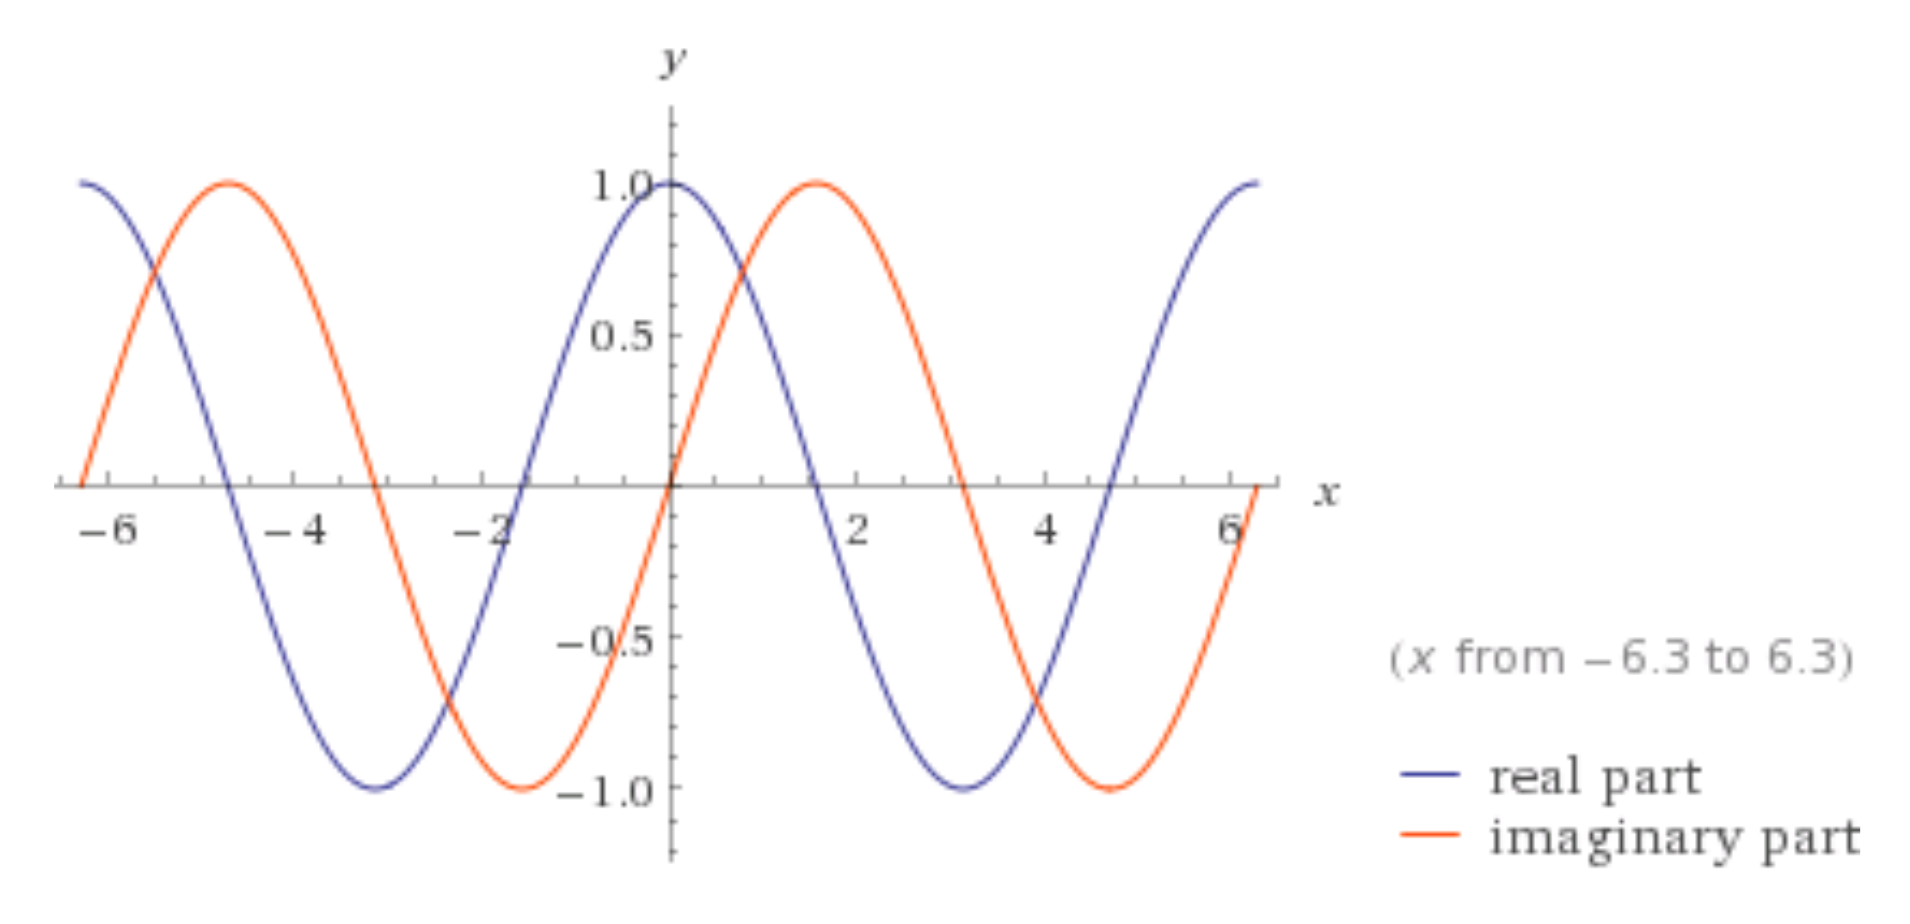
\includegraphics[width = 0.5\textwidth]{exponential.png}
  \caption{Graph of $\exp\left(ix\right)$}
\end{wrapfigure}
이 그래프에서 허수부가 움직이는 곡선을 잘 따라가다 보면 x축과의 교점이 3보다 약간 큰 수라는 것을 알 수 있다. 그리고 파동이 주기를 갖고 진동하고 있음을 볼 수 있다. 이 함수 하나가 $\pi$를 정의하면서도 그 중요성을 설명해 줄 수 있다. 왜 여기서 느닷없이 $\pi$가 등장하는 것일까? \par
이 모든 것의 근간에 있고 $\pi$와 $e$가 보편적으로 나타나는 그 원천에 있는 것이 다음의 간단하기 그지없는, 그렇지만 매우 강력하고도 중요한 방정식이다.
$$
  f' = f
$$
이 간단한 미분방정식의 해가 되는 함수 $f$는 여러 꼴을 가진다. 대표적으로 $f\left(x+c\right)$들도 해가 된다. 미분의 연쇄법칙(Chain rule)을 적용해보면 쉽게 증명할 수 있다. 이와 더불어 상수배를 한 함수의 집합 $\left\{g\;\middle|\; g = kf, \; k\in\mathbb{C}\right\}$도 모두 해가 된다. 이렇게 생각하면 해가 여럿인 것처럼 보인다. 과연 그러할까? \par
아무 상수 $c$를 골라보자. 그리고 $f\left(c\right)f\left(x\right)$와 $f\left(x+c\right)$를 비교해보자. 미분방정식은 초기값을 고정하면 유일한 해를 갖게 된다. $f\left(0\right) = 1$이라고 해보자. 이제 위의 식은 $x = 0$일 때의 값이 같다. 그러므로 $f\left(x\right)f\left(c\right) = f\left(x+c\right)$라고 할 수 있다. 지수 함수에 익숙한 우리들은 이 등식을 보고 지수함수임을 어렵지 않게 눈치 챌 수 있지만, 이러한 유도 과정을 따라가는 것은 이 함수가 그냥 근본없이 튀어나온 게 아닌 저 미분방정식에 근원을 두고 도출된 결과이며, 위와 같은 성질을 가짐을 증명할 수 있기 때문이다. 이 수식은 매우 중요하므로 다시 한번 쓰도록 한다.
\begin{equation}
  f\left(x+y\right) = f\left(x\right)f\left(y\right)
\end{equation}
다시 처음의 미분방정식을 보자. $f'=f$을 만족하는 함수 $f$는 아무 상수 $c$만큼 차이나는 정의역의 값 $x$를 가져와도 모두 해가 되었다. 이제 $f\left(0\right) = 1$로 고정했으니 모든 $x$에 대해 다음의 식을 만족한다:
$$
  f\left(x+c\right) = f\left(x\right)f\left(c\right).
$$
위와 같은 식을 만족하는 $c$를 우리는 `주기'라고 부른다. 그리고 이 주기는 매우 독특한 값을 갖는다. 오일러가 가장 아름답다고 했던 식에서 나오는 $c = 2\pi i$이다. 허수가 붙은 이 수가 중요한 이유는 원래의 미분방정식이 그 어떠한 단위도 갖지 않고 다른 것에 그 근거를 두지 않는 아주 간단하고 독립적인 미분방정식이기 때문이다. 그리고 이제 우리는 $\pi$를 정의할 수 있다. 이 숫자는 $2c i$가 지수함수의 주기가 되게 하는 가장 작은 양의 실수 $c$이다.\par
최근 들어 $\pi$보다 $2\pi$가 더 중요하고 근본적인 의미를 지니므로 이것을 $\tau$라는 상수로 지정해서 사용해야 한다는 움직임이 있다. 틀린 말은 아니다. 유클리드 기하에서 원주와 지름의 비를 계산하는 것은 조금 어색하다. 우리는 지름보다 반지름을 더 많이 사용하기 때문에 원주와 반지름의 비가 더 자연스럽다. 그리고 이는 $2\pi$가 된다. 지수함수의 주기도 $2\pi$이다. 이 성질은 함수 $f$의 푸리에 변환(Fourier transform)을 아래와 같이 정의하면 정규화 상수가 $\left(2\pi\right)^{-1/2}$가 되게 한다:
$$
  \hat{f}\left(\omega\right) = \frac{1}{\sqrt{2\pi}}\int_{-\infty}^{\infty} f\left(x\right)e^{-i\omega x}\, dx.
$$
일반적인 주파수를 사용하더라도
$$
  \hat{f}\left(\omega \right) = \int_{-\infty}^{\infty}f\left(x\right)e^{-2\pi i \omega x}\, dx
$$
가 되어 여전히 $2\pi$가 남는다. 하지만 관례적으로 $\pi$를 많이 써서 이미 굳어진 전통이고 무엇이 정론인가 하는 사소한 문제로 싸우는 것은 수학의 발전에 그다지 도움이 되지 못한다. 더 중요한 것은 이 숫자가 $e$와 어떤 연관성을 가지며 어떻게 도출되는지를 알고 있는가 하는 것이다.
\section{계산가능수(computable numbers)와 $\pi$}
이번 장에서는 초월수(transcendental numbers)와 대수적 수(algebraic numbers)와 조금 다른 수의 집합을 소개한다. 초월수와 대수적 수도 수 체계에서 꽤 중요한 역할을 하고 있지만, 실용성의 측면에서 조금 다른 숫자의 분류가 필요하다. 이제 더이상 인간의 사고 내에서 수학을 하는 시대가 지나가고 본격적으로 컴퓨터를 활용하여 수학을 응용하는 시대가 되어가고 있기 때문이다. 어떠한 수는 컴퓨터로 연산해낼 수 있고 어떠한 수는 연산해낼 수 없다면, 실수 집합 전부를 대상으로 생각하는 것은 의미가 없다. 그 속에서 $\pi$는 어떤 위치에 있는지 알아보도록 하자. \par
수학은 매우 강한 추상성을 지니고 있다. 개념상으로 생각해볼 수 있는 것도 실제로 연산하려고 하면 불가능한 것도 있고 어느 정도의 오차를 감안하더라도 꽤 정확하게 근사할 수 있는 것도 있다. 이미 실수 체계를 구축하고 칸토어(Cantor)가 실수 집합은 불가산이라는 것을 증명한 순간 실수는 인간이 운용할 수 있는 능력의 한계를 벗어난 것이다. 우주에 존재하는 모든 원자를 동원하더라도 실수 집합을 저장하고 만들어낼 수 없다. 그렇기 때문에 어떻게 하면 오차를 최소화하면서 빠르게 연산해낼 수 있을까 하는 것이 중요해졌다. 수학자들 중에서도 실용성을 추구하는 사람들 혹은 실제로 수학을 응용하고 있는 분야의 연구자들, 예를 들어 물리학자나 공학자들은 실수 체계 중에 어디까지 인간이 사용할 수 있는 것인지 생각해보기 시작했다. 컴퓨터의 등장과 함께 이러한 고민은 수치해석이라는 학문으로 집대성되었다. \par
요즘 장안의 화제가 되고 있는 인공지능이라는 개념을 최초로 제시한 사람은 `이미테이션 게임'이라는 영화로도 만들어진 `앨런 튜링(Alan Turing)'이다. 지금은 일상이 되어버린 컴퓨터의 초창기 모델을 생각해낸 사람이기도 하다. 그는 컴퓨터 과학자이자 수학자이기도 했는데 `계산가능수에 대하여(On computable numbers)'라는 논문에서 `계산가능수'를 제시한다. 계산가능수는 유한하고 종국에 끝이 나는 알고리즘으로 원하는 오차한계 이내로 연산해낼 수 있는 실수를 말한다. 이제 어떤 새로운 수를 쓸 때 그 수를 작은 오차로 근사시킬 수 있는지가 중요해졌다. $\pi$는 당연히 계산가능수이다. 하지만 놀라운 것은 계산가능수라는 집합은 아무리 커봤자 가산집합이며 대부분의 실수는 계산가능하지 않다. 그러니까 우리가 쓰는 숫자는 실수 중 극히 일부분이라는 뜻이며 아무리 빠른 컴퓨터로 연산을 해도 대부분의 실수는 영겁의 시간이 지나도 계산해낼 수 없다는 뜻이 되겠다.
\subsection{$\pi$는 어떻게 계산할까}
중등교육을 거쳐 대학에 들어와서 수학을 다시 배우면 그때까지 배운 수학과는 초점이 조금 다르다는 것을 느낀다. `무엇이냐' 이전에 `존재하냐'부터 따지고 존재한다고 해서 곧바로 `무엇이냐'로 넘어가지 않고 `그럼 유일하냐'를 생각한다. 무턱대고 찾지 않는다는 의미이다. $\pi$ 역시 그러한 숫자가 있음을 알았다면 우리가 사용할 수 있는 숫자인지 아는 것이 필요하다. 바로 전에 $\pi$는 계산가능한 수라는 것을 알았으므로 이제는 그러면 어떻게 계산해낼 것인지가 중요해진다.\par역사적으로 $\pi$는 다양한 방법으로 근사되었다. 가장 원시적인 방법으로는 이집트인들이 사용했던 $22/7$이라는 숫자가 있다. 이 숫자는 약 3.142857로 소숫점 아래 2자리까지 정확하므로 그다지 좋은 근사치라고 볼 수 없다. 2세기 무렵의 천체물리학자 프톨레마이오스는 $\pi$의 근사값으로 $377/120$을 썼다. 이것도 약 3.141667로 소숫점 아래 3자리까지 정확하다. 근대적인 수학이 있기 전 사람들은 이와 같이 유리수로 $\pi$를 근사시키려고 노력했다. 근대적인 수학이 어느 정도 자리 잡은 후에는 무한합을 이용하여 계산하려는 노력이 많았다. 이런 무한합 꼴은 `근사'한다고 표현하기에는 부적절하다. 왜냐하면 무한개의 항을 모두 더하면 그 값이 정확히 $\pi$가 되기 때문이다. \par
컴퓨터가 생기고 나서 $\pi$를 더 정확하게 알려는 노력이 있었고, 여러 알고리즘이 개발되었다. 이러한 알고리즘의 기저에는 수렴 속도에 대한 고민이 깔려있다. 이 말인즉슨 컴퓨터로 무한합을 더해 나갈 때 수용할 수 있는 오차 (tolerance)를 정해놓고 그 오차 이하로 내려가면 중단하게 되는데, 이 중단까지 걸리는 시간이 얼마나 길지 생각해 보아야 한다는 것이다. 아래에는 몇 가지 근대적인 알고리즘을 소개한다.
\subsubsection{몬테칼로 방법}
몬테칼로 방법 혹은 몬테칼로 시뮬레이션은 어떤 수치를 계산하는 데에 확률변수의 랜덤성을 이용하는 방법 일체를 이른다. $\pi$ 역시 몬테칼로 방법으로 근사시킬 수 있는데, 이는 $\pi$가 어떤 확률변수의 기댓값으로 표현될 수 있기 때문이다. 확률 변수 $X, Y$가 각각 독립인 Uniform(0,1)을 따른다고 할 때 다음과 같이 정의하자:
$$
  Z = \begin{cases}1, & X^{2} + Y^{2}\leq 1 \\0, & \text{otherwise} \end{cases}.
$$
그러면 $Z$의 기댓값 $\mathbb{E}Z$는 $\pi/4$가 됨을 보일 수 있다. 강대수의 법칙에 따라 $Z$를 무한히 많이 뽑은 후 그것의 산술평균을 내게 되면 $\pi/4$가 된다. 이 과정을 다음과 같은 알고리즘으로 표현할 수 있다.
\begin{algorithm}
  \caption{Monte-Carlo method for $\pi$}
  \begin{algorithmic}[1]
  \Procedure{MCpi}{$\tau$}\label{MCpi}\Comment{$\tau$ is the tolerance}
    \State $n \gets 0$\Comment{set total number to 0}
    \State $c \gets 0$\Comment{set count to 0}
    \State $p_{\text{old}} \gets 0$
    \State $p_{\text{new}} \gets 0$
    \State $\epsilon \gets \tau + 1$
    \While{$\epsilon > \tau$}\Comment{while increment between iterations is greater than the tolerance}
      \State $n \gets n + 1$\Comment{increment on each iteration}
      \State $X \gets \opn{Unif}\left(0,1\right)$
      \State $Y \gets \opn{Unif}\left(0,1\right)$
      \If{$X^{2}+Y^{2} \leq 1$}
        \State $c \gets c + 1$\Comment{count the iteration satisfying the condition}
      \EndIf
      \State $p_{\text{new}} \gets c/n$
      \State $\epsilon \gets p_{\text{new}}-p_{\text{old}} $
      \State $p_{\text{old}} \gets p_{\text{new}}$
    \EndWhile
  \EndProcedure
  \end{algorithmic}
\end{algorithm}

이 방법은 의사코드(pseudocode)이며 어떤 언어로도 옮길 수 있지만 효율적인 코드는 아니다.  그렇다면 이 방법은 좋은 알고리즘인가? 그렇지 않다. 수렴속도가 굉장히 느리다. 매우 흥미로운 근사 방법이긴 하지만 $\pi$의 소숫점 전개를 구할 때 몬테칼로 방법을 쓰지는 않는다. 컴퓨터가 없던 시절, 몬테칼로와 비슷한 방법으로 $\pi$를 구하려고 했던 사람이 있었다. 이를 `뷔퐁의 바늘(Buffon's needle)' 문제라고 부르는데 1901년 이탈리아의 수학자 마리오 라차리니는 똑같은 실험으로 $355/113$이라는 매우 근사한 추정치를 구하였다. 몬테칼로 방법이 지니는 의미는 무리수인 $\pi$를 유리수로 근사시켜 나가는 이른바 `코쉬수열(Cauchy sequence)'의 예로 볼 수 있기 때문이다. 이로써 유리수 집합은 실수 집합에 대해 조밀(dense)하다는 것이 경험적으로 증명된다.

\subsubsection{라마누잔의 방법}
이번에 소개할 알고리즘은 인도의 위대한 수학자 라마누잔이 쓴 방법이며 실제로 PiFast라는 프로그램에서 사용하고 있는 알고리즘이다.
\begin{algorithm}
  \caption{Ramanujan's algorithm for $\pi$}
  \begin{algorithmic}[1]
  \Procedure{RJpi}{$\tau$}\label{RMpi}\Comment{$\tau$ is the tolerance}
    \State $k_{1} \gets 545140134,\; k_{2} \gets 13591409,\; k_{3} \gets 640320, \; k_{4}\gets 100100025, \; k_{5} \gets 327843840, \; k_{6} \gets 53360 $
    \State $\opn{RJpi} \gets 0$
    \State $n \gets 0$
    \State $\epsilon \gets \tau + 1$
    \While{$\epsilon > \tau$}
      \State $\epsilon \gets \left(-1\right)^{n}\frac{\left(6n\right)!\left(k_{2}+nk_{1}\right)}{\left(n!\right)^{3}\left(3n\right)!\left(8k_{4}k_{5}\right)^{n}}$
      \State $\opn{RJpi} \gets \opn{RJpi} + \epsilon$
      \State $n \gets n + 1$
    \EndWhile
    \State $\opn{RJpi} \gets \dfrac{k_{6}\sqrt{k_{3}}}{\opn{RJpi}}$ 
  \EndProcedure
  \end{algorithmic}
\end{algorithm}

라마누잔은 그의 논문 \emph{Modular equations and approximations to} $\boldsymbol{p}$, Quart.J.Pure Appl. Math., (1914), vol. 45, p.350-372에서 위의 알고리즘 도출 과정에 대해 딱히 설명을 하지 않기 때문에 이런 알고리즘을 어떻게 발견했고 저러한 상수 $k_{1},\ldots , k_{6}$까지 어떤 방법으로 생각해냈는지 알 턱이 없다. 하지만 이 알고리즘은 빛의 속도로 $\pi$에 수렴한다. 매 반복시행마다 약 소숫점 아래 14개 자리씩 정확해진다고 하니 놀라울 따름이다.
\end{document}


